\section{Introduction}
Hyperspectral imaging is extremely useful for classifying substances from a distance, but it is also very expensive. This paper will study if it is possible to correlate the data between a camera and a spectrometer. This will be a step towards making it feasible to use the much cheaper combination of camera and spectrometer instead of a hyperspectral camera. The advantage of a hyperspectral camera is that you can get high spectral resolution in combination with high spatial resolution, usually 1 dimension for each. The proposed alternative is one where a camera is combined with a spectrometer. The camera will be able to give high spatial resolution in 2D, while the spectrometer will provide high spectral information for the same sample. This could be a good replacement in ideal situations with homogenous objects, or if the average characteristics of a heterogenous substance is of interest. The theoretical setup is shown in figure \ref{fig:measurement_setup}. 

The postulate to be explored: 
The spatial average across an image of each color, is comparable with the spectral average of a spectrum. That is if that spectrum has been multiplied with the quantum efficiency of each color of the camera sensor. 

Postulates further that the relationship between the values can be found through linear regression. This will have the following uses: 
\begin{itemize}
    \item The regression line can be used to tell if an image and a specter is taken correctly, that they are watching the same object. 
    \item If the previous is known to be true the regression line can give information about noise, from ambient light or other sources. 
\end{itemize}

%TODO: Add the focus which is finding correlating values between camera and spectrometer

\begin{figure}[h]
    \centering
    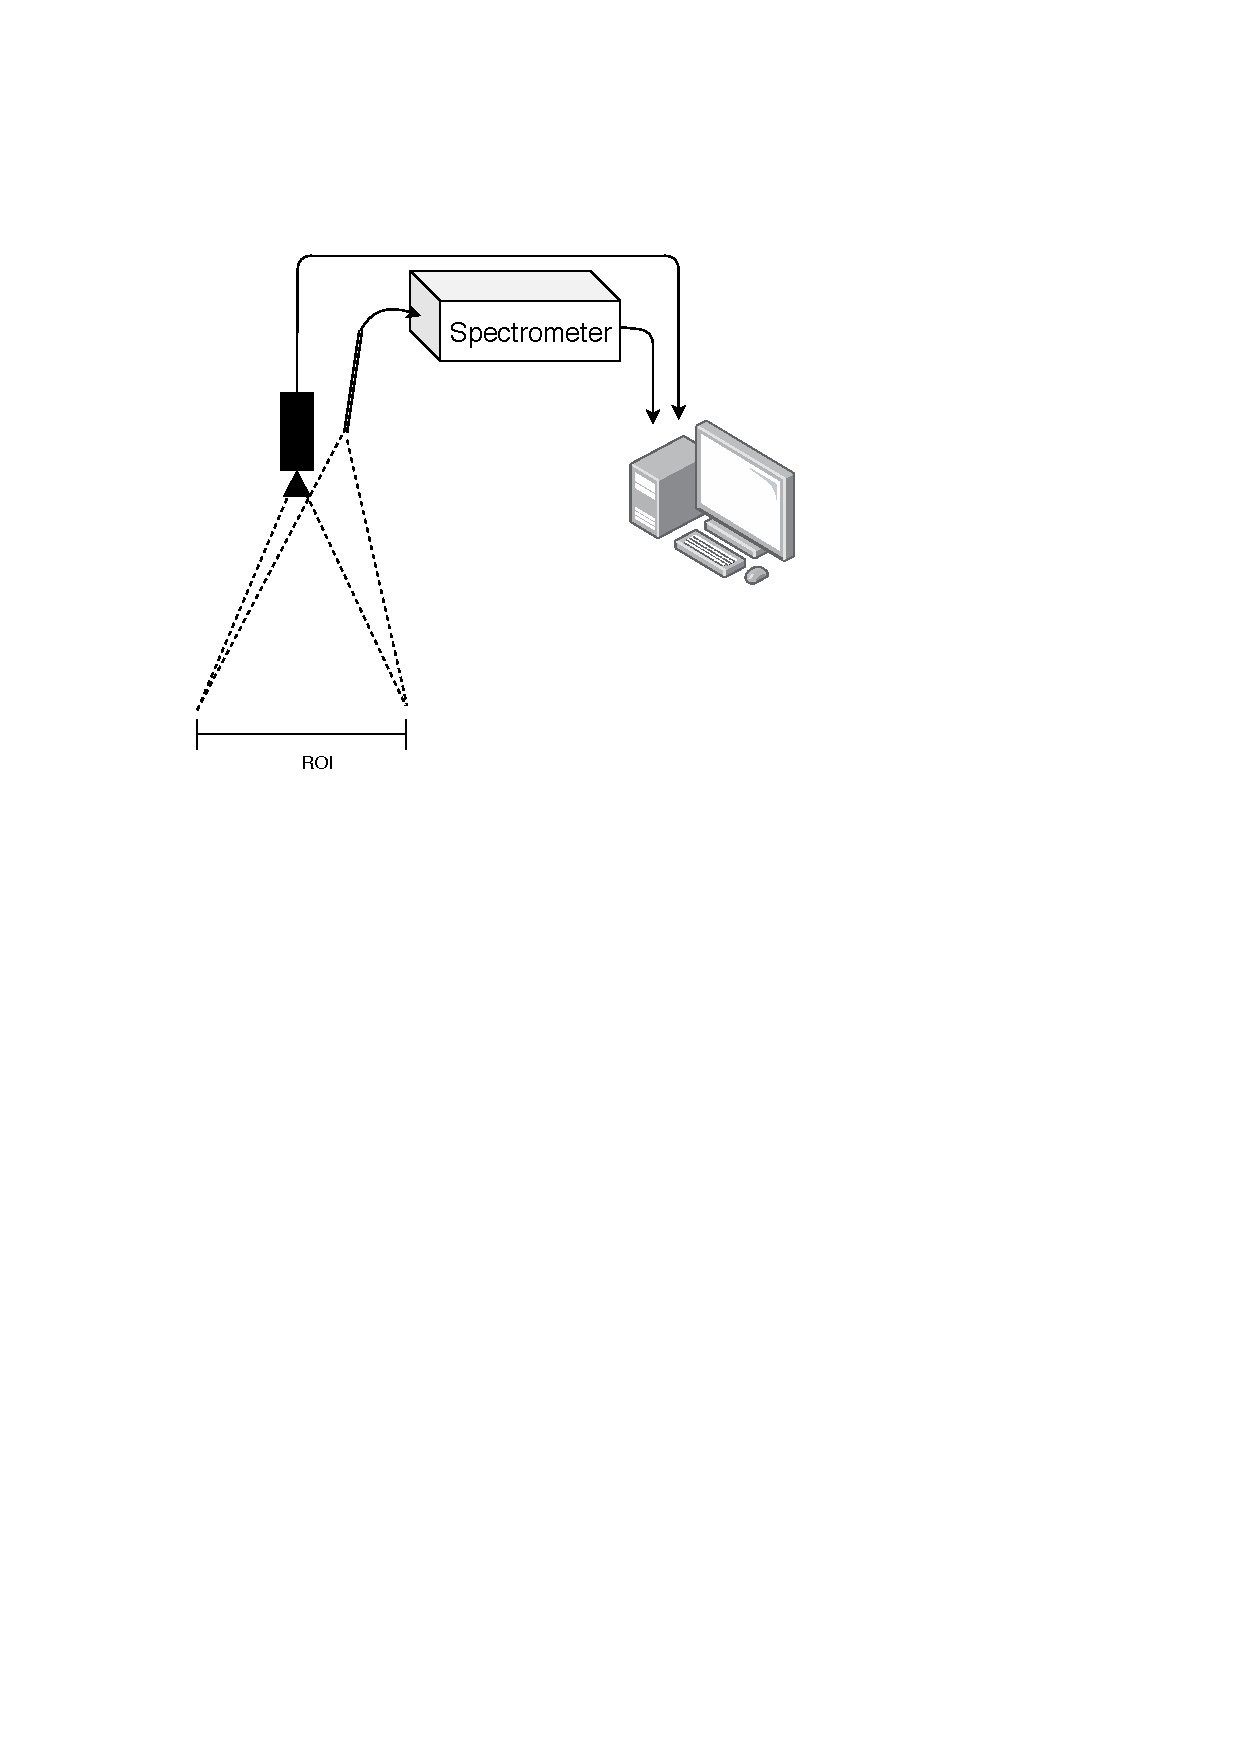
\includegraphics[width=0.5\textwidth]{figures/pt_setup.pdf}
    \caption{Measurement setup}
    \label{fig:measurement_setup}
\end{figure}

